\documentclass[a4paper,12pt]{article}
\usepackage[utf8]{inputenc}
\usepackage[spanish]{babel}
\usepackage{graphicx}
\title{Figuras}
\author{Curso de introducción a LaTeX}
\begin{document}
\maketitle
%Incluir una figura con una leyenda antepuesta:
\begin{figure}[h] 
	\centering
	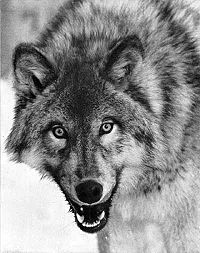
\includegraphics[width=0.2\textwidth]{fig/canis}
	\caption{Una imagen de un lobo.}
\end{figure}

%Incluir una figura con la leyenda al pie de la imagen y con una etiqueta que incluye un seudónimo:
\begin{figure}[h] 
	\centering
	
\includegraphics[width=0.7\linewidth]{fig/php}
	\caption[PHP]{Preprocesor Hypertext}
\end{figure}


La razón porque las figuras son llamadas elementos flotantes (floats), es porque su contenido no será afectado por el texto adyacente ni por el cambio de páginas, apareciendo siempre íntegro en la posición especificada de la página. Los elementos flotantes no son parte del flujo normal del texto, sino que aparecen como entidades separadas, colocados en una parte de la página por sí mismos (superior, medio, inferior, izquierda, derecha, o donde sea que lo definamos en las opciones). 

Para las figuras, esta posición se define dentro de las opciones del entorno figure, pudiendo estar en la parte superior [t], en la base [b], en el lugar en donde se introduce la figura aproximadamente [h] o en una página especial [p]. Este comportamiento se puede apreciar en este ejemplo.

\begin{figure}[h] 
	\centering
	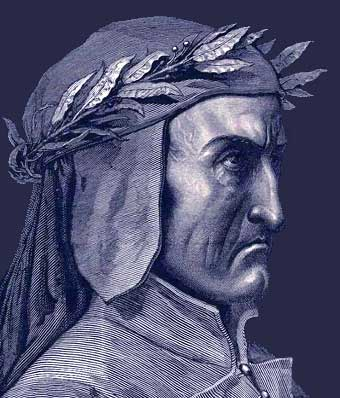
\includegraphics[width=0.2\linewidth]{fig/dante}
	\caption[Dante]{Dante Alighieri}
\end{figure}

Los elementos flotantes existen para hacer frente al problema de los objetos que no caben en la página actual, y para ayudar cuando realmente no deseas preocuparte por la posición del objeto en el documento en ese momento.
\end{document}